\documentclass[11pt,a4paper]{article}

% ── Packages ──────────────────────────────────────────────
\usepackage[margin=2.5cm]{geometry}
\usepackage{graphicx}
\usepackage{booktabs}
\usepackage{enumitem}
\usepackage{xcolor}
\usepackage{listings}
\usepackage{hyperref}
\usepackage{amsmath}
\usepackage{tikz}
\usetikzlibrary{arrows.meta, positioning, shapes.geometric, fit, calc, matrix}
\usepackage{caption}
\usepackage{subcaption}
\usepackage{fancyhdr}
\usepackage[T1]{fontenc}
\usepackage{lmodern}
\usepackage{tabularx}
\usepackage{multirow}
\usepackage{float}

% ── Colors ────────────────────────────────────────────────
\definecolor{codebg}{HTML}{1E1E2E}
\definecolor{codetext}{HTML}{CDD6F4}
\definecolor{accent}{HTML}{E8873A}
\definecolor{accentblue}{HTML}{89B4FA}
\definecolor{green}{HTML}{A6E3A1}
\definecolor{red}{HTML}{F38BA8}
\definecolor{yellow}{HTML}{F9E2AF}
\definecolor{dimtext}{HTML}{6C7086}
\definecolor{layerui}{HTML}{89B4FA}
\definecolor{layercore}{HTML}{A6E3A1}
\definecolor{layermodel}{HTML}{F9E2AF}
\definecolor{layermidi}{HTML}{CBA6F7}
\definecolor{layerhw}{HTML}{F38BA8}
\definecolor{layerrender}{HTML}{94E2D5}

% ── Listings ──────────────────────────────────────────────
\lstset{
  language=C++,
  basicstyle=\ttfamily\footnotesize\color{codetext},
  backgroundcolor=\color{codebg},
  keywordstyle=\color{accentblue}\bfseries,
  commentstyle=\color{dimtext}\itshape,
  stringstyle=\color{green},
  numbers=left,
  numberstyle=\tiny\color{dimtext},
  numbersep=8pt,
  frame=single,
  rulecolor=\color{dimtext},
  breaklines=true,
  tabsize=4,
  showstringspaces=false,
  xleftmargin=1.5em,
  framexleftmargin=1.5em,
  morekeywords={override, nullptr, auto, unique_ptr, string, set, pair, vector, enum, class, struct}
}

% ── Header/Footer ────────────────────────────────────────
\pagestyle{fancy}
\fancyhf{}
\lhead{\small\textit{Gateless Gate --- Erae Touch~II Shape Editor}}
\rhead{\small\textit{George Redpath}}
\cfoot{\thepage}

% ── Hyperlinks ────────────────────────────────────────────
\hypersetup{
  colorlinks=true,
  linkcolor=accent,
  urlcolor=accentblue,
  citecolor=green
}

% ── Title ─────────────────────────────────────────────────
\title{%
  \vspace{-1cm}
  {\Large\textbf{Erae Touch~II Shape Editor}}\\[0.4em]
  {\large A JUCE-Based Visual Layout Editor for\\Multi-Touch Musical Control Surfaces}\\[0.5em]
  \normalsize\textit{Gateless Gate Project --- Thesis Component Report}
}
\author{George Redpath\\[0.2em]
  \small NTNU / Aalborg University}
\date{\today}

% ══════════════════════════════════════════════════════════
\begin{document}
\maketitle
\thispagestyle{fancy}

% ── Abstract ──────────────────────────────────────────────
\begin{abstract}
This document presents the \textbf{Erae Shape Editor}, a 10,016-line JUCE
C++17 application (VST3 and Standalone) that provides a visual layout editor
for the Erae Touch~II multi-touch playing surface. The application enables
musicians to design custom touch layouts on a $42 \times 24$ grid, assign MIDI
behaviors with MPE support, and render layouts in real-time onto the hardware's
LED surface via USB SysEx. Key contributions include a modeless shape editing
paradigm supporting five shape types with full undo/redo, per-finger touch
tracking with 10-color visual feedback, musical intelligence features (scale
quantization, velocity curves, latch modes), and integration points for OSC
and control voltage output. The software forms part of the \textit{Gateless
Gate} project, a modular Eurorack synthesizer combining FPGA-based DSP with
touch-based control surfaces.
\end{abstract}

\tableofcontents
\newpage

% ══════════════════════════════════════════════════════════
\section{Introduction}
\label{sec:intro}

The Erae Touch~II by Embodme is a $42 \times 24$ grid multi-touch instrument
capable of tracking multiple simultaneous finger positions with continuous
pressure sensing. While the manufacturer provides a configuration application,
it is closed-source and limited in its layout design capabilities.

The \textbf{Erae Shape Editor} was developed as a thesis component of the
Gateless Gate project to provide:

\begin{itemize}[nosep]
  \item A fully open visual layout editor with pixel-level precision
  \item Real-time hardware rendering via the Erae~II SysEx API
  \item Five distinct MIDI behavior types including full MPE
  \item Musical features: scale quantization, velocity/pressure curves, latch modes
  \item Integration with external systems via OSC and control voltage output
  \item A modular, undo-capable architecture suitable for professional use
\end{itemize}

The application is built on the JUCE 7.0.9 framework, compiles as both a
VST3 plugin and standalone application, and comprises 51 source files across
7 architectural modules.

\begin{figure}[H]
  \centering
  \includegraphics[width=0.88\textwidth]{screenshot.png}
  \caption{Erae Shape Editor showing a Wicki-Hayden isomorphic keyboard layout
    with 10-finger multitouch tracking, per-finger color palette, and
    real-time hardware surface rendering. The sidebar contains a 7-bit HSV
    color picker, behavior configuration panel, and alignment tools.}
  \label{fig:editor}
\end{figure}


% ══════════════════════════════════════════════════════════
\section{Context: The Gateless Gate Project}
\label{sec:context}

The Gateless Gate is a 104\,HP Eurorack modular synthesizer system built
around a Zynq-7020 FPGA. The project encompasses:

\begin{itemize}[nosep]
  \item \textbf{302 SystemVerilog DSP modules} ($\sim$107,000 lines of gateware)
  \item \textbf{56 audio channels} (28~ADC + 28~DAC) at 96\,kHz/24-bit
  \item \textbf{Patent-pending 1-Wire topology detection} for automatic patch routing
  \item \textbf{JUCE VST3 control surface} for visual patch editing
  \item \textbf{120-channel USB audio} via custom UAC1 firmware on Zynq PS
\end{itemize}

The DSP module library spans classic synthesizer emulations (Buchla, Serge,
Moog, Make Noise, Mutable Instruments), physical modeling (bowed/plucked/blown
instruments), bioacoustic synthesis, video synthesis (73 LZX-inspired modules),
and chiptune emulations (SID, AY-3-8910, NES 2A03, OPL2).

The Erae Shape Editor serves as a \textbf{complementary touch-based control
interface}. Where the Gateless Gate hardware uses physical rotary encoders and
illuminated 3.5\,mm jacks, the Erae Touch~II provides a continuous pressure-
and position-tracking surface. Together, they demonstrate two paradigms for
expressive modular synthesis control: discrete hardware (knobs/jacks) and
continuous touch surfaces.


% ══════════════════════════════════════════════════════════
\section{Architecture}
\label{sec:arch}

The application follows a layered MVC architecture with strict separation
between data model, business logic, and presentation.

\begin{figure}[H]
  \centering
  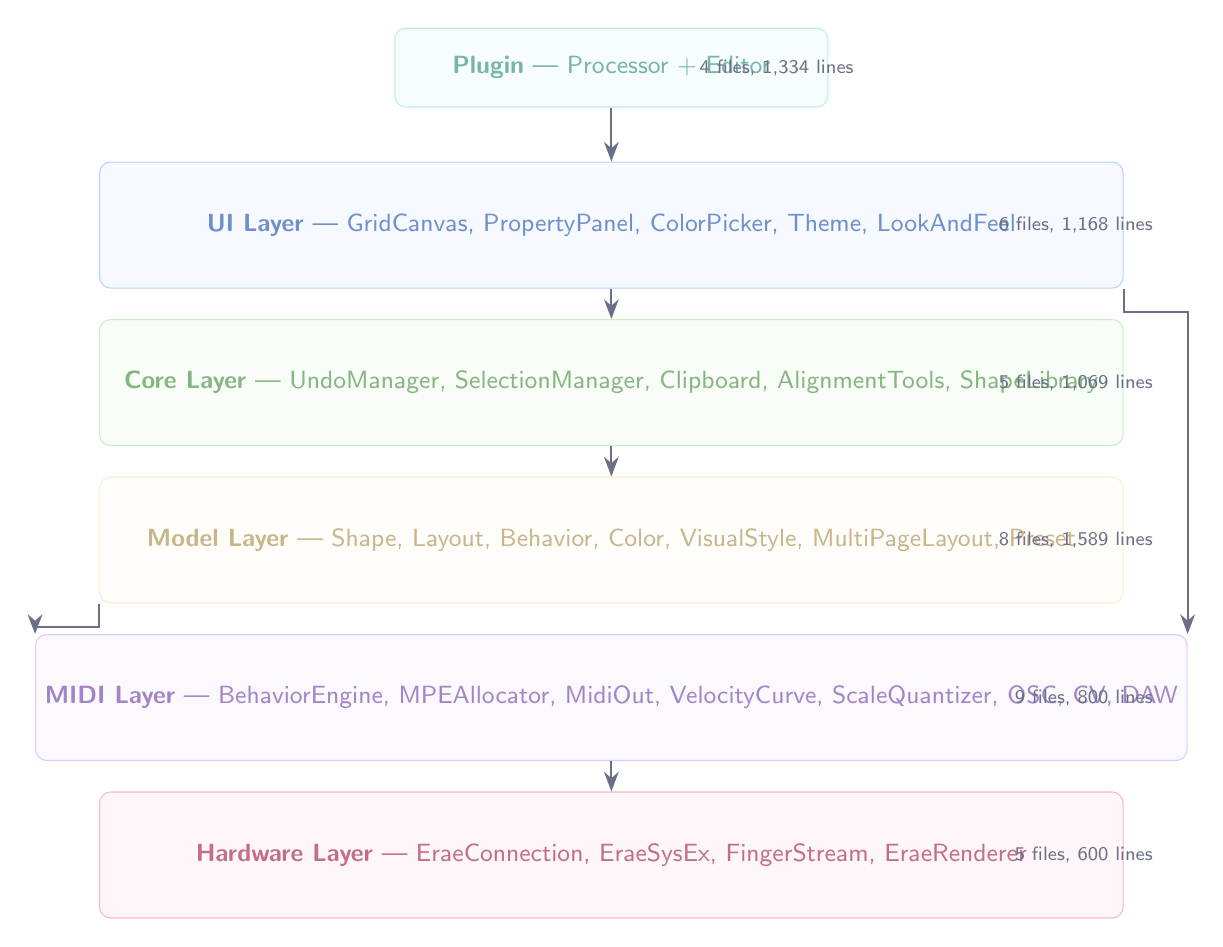
\begin{tikzpicture}[
    layer/.style={rectangle, rounded corners=4pt, minimum width=13cm,
                  minimum height=1.6cm, font=\small\sffamily, draw=#1!60,
                  fill=#1!8, text=#1!80!black},
    file/.style={rectangle, rounded corners=2pt, draw=dimtext, fill=white,
                 font=\scriptsize\ttfamily, inner sep=3pt},
    arrow/.style={-{Stealth[length=2.5mm]}, thick, color=dimtext}
  ]
    % Layers
    \node[layer=layerui]     (ui)     at (0, 8)   {\textbf{UI Layer} --- GridCanvas, PropertyPanel, ColorPicker, Theme, LookAndFeel};
    \node[layer=layercore]   (core)   at (0, 6)   {\textbf{Core Layer} --- UndoManager, SelectionManager, Clipboard, AlignmentTools, ShapeLibrary};
    \node[layer=layermodel]  (model)  at (0, 4)   {\textbf{Model Layer} --- Shape, Layout, Behavior, Color, VisualStyle, MultiPageLayout, Preset};
    \node[layer=layermidi]   (midi)   at (0, 2)   {\textbf{MIDI Layer} --- BehaviorEngine, MPEAllocator, MidiOut, VelocityCurve, ScaleQuantizer, OSC, CV, DAW};
    \node[layer=layerhw]     (hw)     at (0, 0)   {\textbf{Hardware Layer} --- EraeConnection, EraeSysEx, FingerStream, EraeRenderer};

    % Plugin entry
    \node[layer=layerrender, minimum width=5.5cm, minimum height=1cm]
      (plugin) at (0, 10) {\textbf{Plugin} --- Processor + Editor};

    % Arrows
    \draw[arrow] (plugin.south) -- (ui.north);
    \draw[arrow] (ui.south) -- (core.north);
    \draw[arrow] (core.south) -- (model.north);
    \draw[arrow] (ui.south east) -- ++(0,-0.3) -| (midi.north east);
    \draw[arrow] (midi.south) -- (hw.north);
    \draw[arrow] (model.south west) -- ++(0,-0.3) -| (midi.north west);

    % File counts
    \node[font=\scriptsize\sffamily, color=dimtext, anchor=east] at (7, 8) {6 files, 1,168 lines};
    \node[font=\scriptsize\sffamily, color=dimtext, anchor=east] at (7, 6) {5 files, 1,069 lines};
    \node[font=\scriptsize\sffamily, color=dimtext, anchor=east] at (7, 4) {8 files, 1,589 lines};
    \node[font=\scriptsize\sffamily, color=dimtext, anchor=east] at (7, 2) {9 files, 800 lines};
    \node[font=\scriptsize\sffamily, color=dimtext, anchor=east] at (7, 0) {5 files, 600 lines};
    \node[font=\scriptsize\sffamily, color=dimtext, anchor=east] at (3.2, 10) {4 files, 1,334 lines};
  \end{tikzpicture}
  \caption{Layered architecture of the Erae Shape Editor. Arrows indicate
    dependency direction. Line counts include headers and implementations.}
  \label{fig:arch}
\end{figure}

\subsection{Project Statistics}

\begin{table}[H]
  \centering
  \caption{Codebase metrics.}
  \label{tab:stats}
  \begin{tabular}{@{}lr@{}}
    \toprule
    \textbf{Metric} & \textbf{Value} \\
    \midrule
    Total lines of code                    & 10,016 \\
    Source files                           & 51 \\
    Implementation files (.cpp)            & 6,187 lines \\
    Header files (.h)                      & 3,829 lines \\
    Undoable action classes                & 12 \\
    Shape types                            & 5 \\
    MIDI behavior types                    & 5 \\
    Visual animation styles                & 5 \\
    Built-in preset generators             & 6 \\
    Musical scales supported               & 10 \\
    Velocity/pressure curve types          & 4 \\
    Grid resolution                        & $42 \times 24$ (1,008 cells) \\
    Max simultaneous fingers               & 10 (hardware limit) \\
    MPE voice channels                     & 15 (channels 2--16) \\
    CV output channels                     & 32 \\
    Plugin formats                         & VST3 + Standalone \\
    Framework                              & JUCE 7.0.9 \\
    Language standard                      & C++17 \\
    \bottomrule
  \end{tabular}
\end{table}


% ══════════════════════════════════════════════════════════
\section{Model Layer}
\label{sec:model}

\subsection{Shape System}

All coordinates are in grid units ($0$--$41$ horizontal, $0$--$23$ vertical).
The base \texttt{Shape} class defines the interface:

\begin{lstlisting}[caption={Shape base class with virtual geometry methods.}]
struct Shape {
    std::string id;
    ShapeType type;        // Rect, Circle, Hex, Polygon, Pixel
    float x, y;            // reference point
    Color7 color, colorActive;
    std::string behavior;  // "trigger", "momentary", etc.
    juce::var behaviorParams;
    int zOrder;
    std::string visualStyle;

    virtual BBox bbox() const = 0;
    virtual bool contains(float px, float py) const = 0;
    virtual std::vector<std::pair<int,int>> gridPixels() const = 0;
    virtual std::unique_ptr<Shape> clone() const = 0;
    virtual juce::var toVar() const;  // JSON serialization
};
\end{lstlisting}

Five concrete shape types are implemented:

\begin{table}[H]
  \centering
  \caption{Shape types and their storage representation.}
  \label{tab:shapes}
  \begin{tabular}{@{}llll@{}}
    \toprule
    \textbf{Type} & \textbf{Reference Point} & \textbf{Parameters} & \textbf{Hit Test} \\
    \midrule
    Rectangle & Top-left corner   & width, height           & AABB containment \\
    Circle    & Center            & radius                  & Distance $\le r$ \\
    Hexagon   & Center            & radius (flat-top)       & Point-in-polygon (6 vertices) \\
    Polygon   & Origin (min x,y)  & Relative vertex list    & Ray-casting PIP \\
    Pixel     & Origin (min x,y)  & Relative cell set       & Linear cell search \\
    \bottomrule
  \end{tabular}
\end{table}

Every shape provides \texttt{gridPixels()}, which rasterizes the shape to
integer grid coordinates. This is used for both screen rendering and hardware
pixel output. The rasterization is consistent across all types: rectangles fill
their integer bounds, circles test center-of-cell distance, hexagons and
polygons use ray-casting at cell centers, and pixel shapes return their stored
cells directly.

\subsection{Color System}

The Erae Touch~II hardware uses 7-bit RGB color (0--127 per channel). The
\texttt{Color7} struct provides this natively:

\begin{lstlisting}
struct Color7 {
    int r = 0, g = 0, b = 0;
    juce::Colour toJuceColour() const {
        return juce::Colour((uint8)(r * 2), (uint8)(g * 2), (uint8)(b * 2));
    }
};
\end{lstlisting}

The $\times 2$ conversion maps the 7-bit hardware range to 8-bit display
range. An HSV-to-7-bit-RGB converter is provided for the color picker, along
with pitch-class coloring (\texttt{noteColor(note)}: $30^\circ$ hue rotation
per semitone) and utility functions (\texttt{dim()}, \texttt{brighten()}).

\subsection{Layout and Multi-Page}

The \texttt{Layout} class is the single source of truth for one page of
shapes. It provides z-ordered hit testing (reverse-iteration for top-to-bottom
priority), mutation methods with listener notification, and auto-assignment of
MIDI notes and CCs to prevent duplicates.

\texttt{MultiPageLayout} wraps up to 8 layouts (matching the Erae~II firmware
limit) with page navigation, duplication, and JSON serialization. The file
format auto-detects v1 (single-page, no version key) and v2 (multi-page with
\texttt{"version": 2}).

\subsection{Preset System}

Six built-in preset generators create common musical layouts:

\begin{table}[H]
  \centering
  \caption{Built-in preset generators.}
  \label{tab:presets}
  \begin{tabular}{@{}llp{6.5cm}@{}}
    \toprule
    \textbf{Preset} & \textbf{Shape Type} & \textbf{Description} \\
    \midrule
    Drum Pads       & Rectangle  & $4 \times 4$ MPC-style grid with chromatic HSV coloring, auto-assigned notes \\
    Piano           & Rectangle  & 3-octave keyboard with white/black keys and z-ordered layering \\
    Wicki-Hayden    & Hexagon    & $6 \times 10$ isomorphic hexagonal note grid (configurable rows/cols) \\
    Fader Bank      & Rectangle  & 8 vertical faders with rainbow hue distribution, CC 1--8 \\
    XY Pad          & Rectangle  & Single full-surface XY controller \\
    Buchla Thunder  & Mixed      & Faithful Buchla Thunder recreation: 4 trigger buttons, 10 feather polygons, 2 tail pads, 4 palm hexagons (148 lines of geometry) \\
    \bottomrule
  \end{tabular}
\end{table}


% ══════════════════════════════════════════════════════════
\section{Core Services}
\label{sec:core}

\subsection{Undo/Redo System}

The undo system implements the Command pattern with 12 concrete action types:

\begin{table}[H]
  \centering
  \caption{Undoable action classes. Actions marked with $\star$ support drag coalescing.}
  \label{tab:actions}
  \begin{tabular}{@{}ll@{}}
    \toprule
    \textbf{Action} & \textbf{Purpose} \\
    \midrule
    \texttt{AddShapeAction}       & Add a new shape to the layout \\
    \texttt{RemoveShapeAction}    & Delete a single shape \\
    \texttt{RemoveMultipleAction} & Delete multiple selected shapes \\
    \texttt{MoveShapeAction}$^\star$      & Move a single shape \\
    \texttt{MoveMultipleAction}$^\star$   & Move multiple shapes by same delta \\
    \texttt{ResizeRectAction}$^\star$     & Resize rectangle via handles \\
    \texttt{ResizeCircleAction}$^\star$   & Resize circle radius \\
    \texttt{ResizeHexAction}$^\star$      & Resize hexagon radius \\
    \texttt{SetColorAction}       & Change shape colors \\
    \texttt{SetBehaviorAction}    & Change MIDI behavior and parameters \\
    \texttt{SetShapesAction}      & Replace all shapes (preset loading) \\
    \texttt{AlignAction}          & Alignment tool moves \\
    \texttt{EditShapeAction}      & In-place shape geometry editing \\
    \bottomrule
  \end{tabular}
\end{table}

\textbf{Drag coalescing} is a key optimization: during a mouse drag that
generates many incremental move/resize actions, consecutive actions with the
same \texttt{dragId} are merged so that a single Ctrl+Z undoes the entire drag
rather than each pixel increment.

\begin{lstlisting}[caption={Drag coalescing via unique drag IDs.}]
bool MoveShapeAction::canCoalesceWith(const UndoableAction& other) const {
    if (dragId_ == 0) return false;
    auto* o = dynamic_cast<const MoveShapeAction*>(&other);
    return o && o->dragId_ == dragId_ && o->id_ == id_;
}
\end{lstlisting}

\subsection{Selection and Clipboard}

The \texttt{SelectionManager} tracks a set of selected shape IDs with
single-select, multi-select (Shift+click toggle), and select-all operations.
The \texttt{Clipboard} provides copy/cut/paste with automatic position offset,
new ID assignment, and MIDI note/CC deconfliction for duplicated shapes.

\subsection{Alignment Tools}

When two or more shapes are selected, eight alignment operations become
available: align left/right/top/bottom, center horizontally/vertically,
and distribute horizontally/vertically. Each operates on bounding boxes and
generates an \texttt{AlignAction} for undo support.

\subsection{Shape Library}

Users can save any shape to a persistent library stored at
\texttt{\textasciitilde/.EraeShapeEditor/library.json}. Library entries
preserve full shape state (geometry, color, behavior, visual style) and can
be placed onto the canvas, flipped horizontally or vertically, and deleted.
The library persists across sessions.


% ══════════════════════════════════════════════════════════
\section{MIDI and Musical Intelligence}
\label{sec:midi}

\subsection{Behavior Engine}

The \texttt{BehaviorEngine} is a state machine that routes
\texttt{FingerEvent}s to behavior-specific handlers based on the touched
shape's configuration:

\begin{figure}[H]
  \centering
  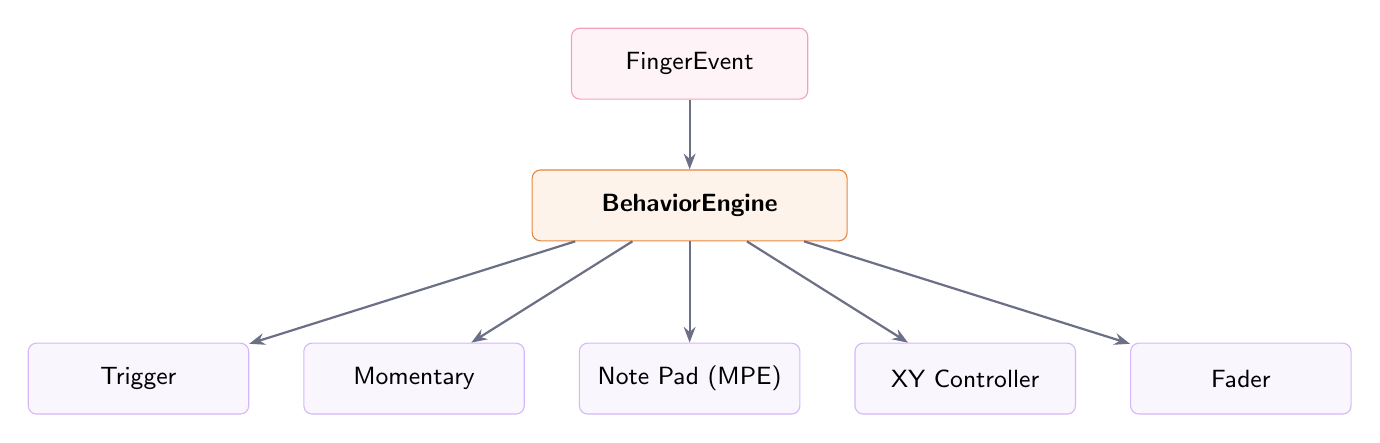
\begin{tikzpicture}[
    beh/.style={rectangle, rounded corners=3pt, draw=layermidi!80, fill=layermidi!10,
                text=black, font=\small\sffamily, minimum width=2.8cm, minimum height=0.9cm},
    arrow/.style={-{Stealth[length=2mm]}, thick, color=dimtext}
  ]
    \node[beh] (trigger)   at (0, 0)    {Trigger};
    \node[beh] (momentary) at (3.5, 0)  {Momentary};
    \node[beh] (notepad)   at (7, 0)    {Note Pad (MPE)};
    \node[beh] (xy)        at (10.5, 0) {XY Controller};
    \node[beh] (fader)     at (14, 0)   {Fader};

    \node[rectangle, rounded corners=3pt, draw=accent, fill=accent!10,
          font=\small\sffamily\bfseries, minimum width=4cm, minimum height=0.9cm]
      (engine) at (7, 2.2) {BehaviorEngine};

    \node[rectangle, rounded corners=3pt, draw=layerhw!80, fill=layerhw!10,
          font=\small\sffamily, minimum width=3cm, minimum height=0.9cm]
      (finger) at (7, 4) {FingerEvent};

    \draw[arrow] (finger) -- (engine);
    \draw[arrow] (engine) -- (trigger);
    \draw[arrow] (engine) -- (momentary);
    \draw[arrow] (engine) -- (notepad);
    \draw[arrow] (engine) -- (xy);
    \draw[arrow] (engine) -- (fader);
  \end{tikzpicture}
  \caption{BehaviorEngine routes finger events to behavior-specific handlers.}
  \label{fig:behavior}
\end{figure}

\begin{table}[H]
  \centering
  \caption{MIDI behavior types and their output.}
  \label{tab:behaviors}
  \begin{tabular}{@{}lp{9cm}@{}}
    \toprule
    \textbf{Behavior} & \textbf{MIDI Output} \\
    \midrule
    Trigger      & Note on/off on touch down/up. Configurable velocity (fixed or pressure-mapped), velocity curve, latch mode (toggle per press). \\
    Momentary    & Note on while held, off on release. Independent velocity and aftertouch pressure curves. \\
    Note Pad     & Full MPE: per-finger channel allocation (channels 2--16), pitch bend from X position, slide CC from Y, channel pressure from Z. Optional scale quantization with glide. \\
    XY Controller & Two CC values from finger X/Y position. Supports 7-bit or 14-bit hi-res mode with configurable min/max output range per axis. \\
    Fader        & Single CC from finger position along one axis. Horizontal or vertical orientation. 7-bit or 14-bit with configurable range. \\
    \bottomrule
  \end{tabular}
\end{table}

\subsection{MPE Allocation}

The \texttt{MPEAllocator} manages per-finger channel assignment across
channels 2--16 (15 MPE voice channels, with channel 1 as the master).
Allocation uses a timestamp-based oldest-steal strategy when all channels
are in use.

\subsection{Scale Quantization}

Ten musical scales are supported for Note Pad mode:

\begin{center}
\small
Chromatic, Major, Natural Minor, Harmonic Minor, Pentatonic,\\
Minor Pentatonic, Whole Tone, Blues, Dorian, Mixolydian
\end{center}

The quantizer operates on both discrete notes
(\texttt{quantizeNote()}) and continuous pitch bend
(\texttt{quantizePitchBend()}). Pitch bend quantization includes an adjustable
glide parameter (0--100\,ms) that blends between the raw and quantized pitch
for expressive portamento between scale degrees.

\subsection{Velocity and Pressure Curves}

Four curve types are available for velocity and pressure mapping, applied
independently:

\begin{table}[H]
  \centering
  \caption{Velocity/pressure curve transfer functions ($x \in [0,1]$).}
  \label{tab:curves}
  \begin{tabular}{@{}lll@{}}
    \toprule
    \textbf{Curve} & \textbf{Function} & \textbf{Character} \\
    \midrule
    Linear      & $f(x) = x$            & Neutral \\
    Exponential & $f(x) = x^3$          & Favors light taps \\
    Logarithmic & $f(x) = 1-(1-x)^3$    & Favors hard presses \\
    S-Curve     & $f(x) = 3x^2 - 2x^3$  & Gentle at extremes (smoothstep) \\
    \bottomrule
  \end{tabular}
\end{table}


% ══════════════════════════════════════════════════════════
\section{Hardware Integration}
\label{sec:hardware}

\subsection{Erae~II SysEx Protocol}

Communication with the Erae Touch~II uses MIDI System Exclusive messages.
The protocol implements a 7-bit encoding scheme where 7~data bytes are packed
into 8~MIDI bytes (7~payload + 1~MSB collector), with a checksum byte for
integrity.

\begin{table}[H]
  \centering
  \caption{Key SysEx commands used by the editor.}
  \label{tab:sysex}
  \begin{tabular}{@{}llp{6cm}@{}}
    \toprule
    \textbf{Command} & \textbf{ID} & \textbf{Description} \\
    \midrule
    API Mode Enable     & \texttt{0x01} & Enter API mode (overrides built-in layout) \\
    API Mode Disable    & \texttt{0x02} & Return to built-in layout \\
    Zone Boundary Req.  & \texttt{0x10} & Query zone dimensions \\
    Clear Zone          & \texttt{0x20} & Clear all pixels in zone \\
    Draw Pixel          & \texttt{0x21} & Set single pixel RGB \\
    Draw Rectangle      & \texttt{0x22} & Fill rectangular region \\
    Draw Image          & \texttt{0x23} & Bulk pixel transfer (chunked by 24 rows) \\
    \bottomrule
  \end{tabular}
\end{table}

\subsection{Fingerstream Parsing}

Incoming finger events are parsed from SysEx messages containing:
\begin{itemize}[nosep]
  \item Action byte (0=down, 1=move, 2=up) and zone ID
  \item 64-bit finger ID (little-endian)
  \item Three 32-bit floats: X position, Y position, Z pressure
\end{itemize}

The parser extracts these from the 7-bit-encoded payload and dispatches
\texttt{FingerEvent} structs to the \texttt{BehaviorEngine}.

\subsection{Auto-Reconnection}

The \texttt{EraeConnection} implements a timer-based auto-reconnect strategy.
Every 3\,seconds it scans available MIDI ports for the Erae~II's ``Lab'' output
and ``Main'' input ports. On connection, the API mode is enabled automatically;
on disconnect, the connection state is reset and scanning resumes. This
provides a seamless plug-and-play experience.

\subsection{Real-Time Surface Rendering}

The \texttt{EraeRenderer} implements a dirty-flag optimized rendering pipeline
at $\sim$20\,fps:

\begin{enumerate}[nosep]
  \item A \texttt{dirty\_} flag is set when the layout changes or finger
        states update. The timer callback is a no-op when nothing has changed.
  \item A $42 \times 24 \times 3$ framebuffer (\texttt{uint8\_t fb[H][W][3]})
        is constructed using a painter's algorithm: shapes are rendered in
        z-order, with later shapes overwriting earlier ones.
  \item For each shape, \texttt{WidgetRenderer::renderWidget()} generates
        per-pixel color commands based on the visual style and current
        \texttt{WidgetState} (finger position, pressure).
  \item DAW feedback highlights are composited by brightening matching shape
        pixels (R+40, G+30, B+5).
  \item Per-finger dots are composited using the 10-color palette from
        \texttt{FingerPalette}.
  \item The Y-axis is flipped for hardware orientation (hardware Y=0 is bottom).
  \item The framebuffer is transmitted as a single \texttt{drawImage()} SysEx
        command (no \texttt{clearZone} to avoid visual flashing).
  \item \texttt{lastWidgetStates\_} is compared to detect state changes without
        triggering unnecessary full redraws.
\end{enumerate}

Five visual animation styles are supported:
\begin{itemize}[nosep]
  \item \textbf{Static} --- Solid color fill
  \item \textbf{Pressure Glow} --- Intensity tracks finger pressure
  \item \textbf{Fill Bar} --- Vertical/horizontal fill follows finger position
  \item \textbf{Position Dot} --- Bright dot tracks finger within shape
  \item \textbf{Radial Arc} --- Arc sweeps based on finger angle from center
\end{itemize}


% ══════════════════════════════════════════════════════════
\section{User Interface}
\label{sec:ui}

\subsection{Layout}

The editor window ($1440 \times 860$ default) is divided into four regions:

\begin{table}[H]
  \centering
  \caption{UI layout regions.}
  \label{tab:uilayout}
  \begin{tabular}{@{}llp{7cm}@{}}
    \toprule
    \textbf{Region} & \textbf{Size} & \textbf{Contents} \\
    \midrule
    Toolbar      & 40\,px high   & Tool buttons, preset selector, brush size, page nav, undo/redo, file I/O \\
    Canvas       & Fills center  & Shape grid ($42 \times 24$ at 20\,px/cell, zoomable 0.25x--4x) \\
    Sidebar      & 270\,px wide  & Color picker, property panel, alignment tools, shape library, OSC settings \\
    Status Bar   & 24\,px high   & Shape count, tool mode, connection status, page indicator \\
    \bottomrule
  \end{tabular}
\end{table}

\subsection{Drawing Tools}

Eight drawing tools are available via toolbar buttons or keyboard shortcuts:

\begin{table}[H]
  \centering
  \caption{Drawing tools and keyboard shortcuts.}
  \label{tab:tools}
  \begin{tabular}{@{}llp{7cm}@{}}
    \toprule
    \textbf{Tool} & \textbf{Key} & \textbf{Interaction} \\
    \midrule
    Select      & V & Click to select, drag to move, handles to resize. Shift+click for multi-select. \\
    Paint       & B & Brush-based pixel painting (size 1--5). Creates 1$\times$1 trigger shapes. \\
    Erase       & E & Removes shapes at cursor position. \\
    Rectangle   & R & Click+drag to define corners. \\
    Circle      & C & Click+drag to define bounding box. \\
    Hexagon     & H & Click+drag for flat-top hexagon. \\
    Polygon     & P & Click vertices, double-click or Enter to close. \\
    Pixel       & G & Paint freeform cells. Right-click to erase. Ctrl+Z undoes last stroke. Enter to finalize. \\
    \bottomrule
  \end{tabular}
\end{table}

\subsection{Edit Shape Mode}

A right-click context menu on any shape in Select mode provides an
\textbf{Edit Shape} option that enters a modeless editing state:

\begin{itemize}[nosep]
  \item \textbf{Left-click/drag}: paint cells onto the shape
  \item \textbf{Right-click/drag}: erase cells from the shape
  \item \textbf{Handle drag}: scale all cells proportionally
\end{itemize}

Non-pixel shapes are auto-converted to \texttt{PixelShape} on first cell edit,
preserving all visual properties. The entire session commits as a single undo
action on exit (ESC or click outside).

\subsection{Color Picker}

A custom 7-bit HSV color picker is optimized for the Erae~II's native color
space. It provides a horizontal hue bar, a saturation-value square, an RGB
readout, and a 16-color quick palette---all producing \texttt{Color7} values
directly without 8-bit intermediaries.

\subsection{Per-Finger Visualization}

The canvas overlays live finger positions received from the Erae~II hardware.
Each of up to 10 simultaneous fingers is drawn with a distinct color from a
perceptually-spaced palette (red, green, blue, yellow, magenta, cyan, orange,
purple, white, lime), a pressure-scaled radius, and a numbered label. This
provides immediate visual feedback during performance.

\subsection{Shape Library}

Users can save any shape to a persistent reusable library stored at
\texttt{\textasciitilde/.EraeShapeEditor/library.json}. Library operations
include:

\begin{itemize}[nosep]
  \item \textbf{Save}: Clone the selected shape into the library with a name
  \item \textbf{Place}: Instantiate a library shape onto the canvas with a new ID
  \item \textbf{Flip Horizontal/Vertical}: Transform the shape geometry
        (polygon vertex mirroring, pixel cell reflection) while preserving
        symmetric shapes (rect, circle, hex) unchanged
  \item \textbf{Delete}: Remove entries from the library
\end{itemize}

The library persists across sessions via JSON serialization and is displayed
in a scrollable list in the sidebar.

\subsection{DAW Feedback}

When running as a VST3 plugin, incoming MIDI note-on/off messages from the DAW
are matched against shape note assignments. Matching shapes receive a pulsing
amber glow overlay on the canvas, and the corresponding hardware pixels are
brightened on the Erae~II surface. This provides visual feedback during
sequenced playback on both the screen and the physical instrument.


% ══════════════════════════════════════════════════════════
\section{External Integration}
\label{sec:integration}

\subsection{OSC Output}

All MIDI output is optionally mirrored as OSC messages over UDP:

\begin{table}[H]
  \centering
  \caption{OSC message addresses and arguments.}
  \label{tab:osc}
  \begin{tabular}{@{}ll@{}}
    \toprule
    \textbf{Address} & \textbf{Arguments} \\
    \midrule
    \texttt{/erae/note/on}   & channel, note, velocity \\
    \texttt{/erae/note/off}  & channel, note \\
    \texttt{/erae/cc}        & channel, controller, value \\
    \texttt{/erae/pressure}  & channel, value \\
    \texttt{/erae/pitchbend} & channel, value \\
    \texttt{/erae/finger}    & fingerId, x, y, z, shapeId \\
    \bottomrule
  \end{tabular}
\end{table}

This enables integration with TouchDesigner, Max/MSP, SuperCollider, and other
OSC-capable environments.

\subsection{Control Voltage Output}

Each shape can optionally output CV signals on the plugin's audio output
channels (channels 2+, after the stereo main bus). The CV system uses the
1\,V/oct standard: MIDI note $0 = 0.0$\,V, note $60 = 5.0$\,V. Per-behavior
channel mapping provides gate, pitch, pressure, and slide signals:

\begin{table}[H]
  \centering
  \caption{CV channel mapping by behavior type.}
  \label{tab:cv}
  \begin{tabular}{@{}lllll@{}}
    \toprule
    \textbf{Behavior} & \textbf{Base+0} & \textbf{Base+1} & \textbf{Base+2} & \textbf{Base+3} \\
    \midrule
    Trigger     & Gate     & Pitch  & ---      & --- \\
    Momentary   & Gate     & Pitch  & Pressure & --- \\
    NotePad     & Gate     & Pitch  & Pressure & Slide Y \\
    XY Ctrl     & X (0--1) & Y (0--1) & ---    & --- \\
    Fader       & Value    & ---    & ---      & --- \\
    \bottomrule
  \end{tabular}
\end{table}

This bridges the touch surface to modular synth environments via DC-coupled
audio interfaces, or directly to the Gateless Gate's 120-channel USB audio
system on the Zybo FPGA.


% ══════════════════════════════════════════════════════════
\section{Theme and Visual Design}
\label{sec:theme}

The application uses a dark theme inspired by professional music production
software (Ableton Live, Bitwig Studio, Vital synthesizer):

\begin{itemize}[nosep]
  \item \textbf{Background}: Dark charcoal (\texttt{\#1E1E2E}) with subtle
        grid lines
  \item \textbf{Accent}: Warm amber (\texttt{\#E8873A}) for selection,
        handles, and active elements
  \item \textbf{Grid}: Major lines every 6 cells (matching Erae~II zone
        boundaries)
  \item \textbf{Typography}: 10--11.5\,pt with bold section headers
  \item \textbf{Spacing}: 4-level scale (4/8/12/16\,px)
  \item \textbf{Handles}: 8\,px rounded rectangles with filled interior
        and border ring
\end{itemize}

A custom \texttt{LookAndFeel} subclass overrides JUCE's default widget
rendering for buttons, sliders, combo boxes, popup menus, toggles, labels,
tooltips, and scrollbars---ensuring visual consistency throughout the
application.


% ══════════════════════════════════════════════════════════
\section{Thread Safety}
\label{sec:threading}

The plugin runs across multiple threads: the GUI message thread, the audio
processing thread, and the MIDI input callback thread. Thread safety is
ensured through:

\begin{itemize}[nosep]
  \item \textbf{SpinLock} protection for: MIDI output queue, CV channel
        buffer, DAW feedback state, OSC socket, finger event listener list
  \item \textbf{Atomic operations} for connection state flags
  \item \textbf{Lock-free patterns} for the CV output buffer (32-channel
        float array with per-channel atomic writes)
  \item \textbf{Message-thread-only} mutations for Layout and UI state,
        enforced by JUCE's \texttt{MessageManagerLock}
\end{itemize}


% ══════════════════════════════════════════════════════════
\section{Keyboard Shortcuts}
\label{sec:shortcuts}

\begin{table}[H]
  \centering
  \caption{Complete keyboard shortcut reference.}
  \label{tab:shortcuts}
  \begin{tabular}{@{}ll@{}}
    \toprule
    \textbf{Shortcut} & \textbf{Action} \\
    \midrule
    Ctrl+Z / Ctrl+Shift+Z & Undo / Redo \\
    Ctrl+A         & Select all shapes \\
    Ctrl+C / X / V & Copy / Cut / Paste \\
    Ctrl+D         & Duplicate selection \\
    Delete          & Delete selection \\
    Arrow keys     & Nudge selected (Shift = 5\,px) \\
    V / B / E / R / C / H / P / G & Tool shortcuts \\
    Enter          & Finalize polygon or pixel shape \\
    Escape         & Cancel creation / exit Edit Shape \\
    Right-click    & Context menu (Edit Shape) \\
    Scroll wheel   & Zoom in/out \\
    Middle-click drag & Pan canvas \\
    \bottomrule
  \end{tabular}
\end{table}


% ══════════════════════════════════════════════════════════
\section{File Format}
\label{sec:format}

Layouts are persisted as JSON. The v2 multi-page format:

\begin{lstlisting}[language={}]
{
  "version": 2,
  "pages": [
    { "shapes": [
        { "id": "shape_1", "type": "rect",
          "x": 5, "y": 3, "width": 4, "height": 3,
          "color": [0, 80, 127],
          "color_active": [127, 127, 127],
          "behavior": "trigger",
          "behavior_params": { "note": 60, "channel": 0 },
          "z_order": 0,
          "visual_style": "pressure_glow" }
    ] }
  ]
}
\end{lstlisting}

Single-page v1 files (no \texttt{"version"} key) are auto-detected and loaded
as a single page, ensuring backward compatibility.


% ══════════════════════════════════════════════════════════
\section{Relation to Thesis}
\label{sec:thesis}

The Erae Shape Editor contributes to the thesis along several dimensions:

\paragraph{Touch Interface Design for Electronic Music.}
The editor demonstrates a shape-semantic approach to touch surface programming,
where geometric primitives carry musical meaning (behavior, pitch, channel) and
visual feedback (animation style, color). This contrasts with both the
manufacturer's fixed-layout approach and traditional MIDI learn workflows.
The five visual animation styles (pressure glow, fill bar, position dot,
radial arc, static) provide real-time haptic-visual feedback that enhances
performer awareness of their gestural input.

\paragraph{Software Engineering for Real-Time Music Systems.}
The command-pattern undo system with drag coalescing, thread-safe MIDI pipeline,
7-bit SysEx encoding layer, and dirty-flag optimized rendering pipeline
illustrate the engineering challenges of building responsive, correct, and
musically useful software that bridges desktop UI with embedded hardware.
The application demonstrates that a 10,000-line codebase with clean MVC
separation can deliver professional-grade functionality.

\paragraph{Musical Intelligence.}
The scale quantization system (10 scales with adjustable glide), MPE
allocation (15 voices across channels 2--16), four velocity/pressure curve
types, and latch modes represent a layer of musical intelligence that
transforms raw touch data into expressive MIDI output. These features
are typically found only in commercial products.

\paragraph{Multi-Protocol Output.}
The simultaneous MIDI, OSC, and CV output paths demonstrate that a single
touch event can drive multiple downstream systems: a DAW (via MIDI/VST3),
a visual environment like TouchDesigner (via OSC/UDP), and a modular
synthesizer (via CV on audio channels). This multi-protocol approach enables
the Erae~II to serve as a universal controller in hybrid setups.

\paragraph{Integration with the Gateless Gate Ecosystem.}
The CV output system directly bridges the touch surface to the Gateless Gate's
FPGA-based DSP engine via 120-channel USB audio. Scale quantization and MPE
support align with the modular synthesis paradigm, making the Erae~II a viable
performance controller for the hardware synthesizer. The DAW feedback loop---
where MIDI notes from the Gateless Gate's sequencer illuminate the
corresponding touch pads---closes the visual feedback circuit between
performer and instrument.

\paragraph{Open-Source Alternative.}
The application provides an open-source alternative to the manufacturer's
closed-source configuration tool, with additional capabilities (CV output,
OSC, shape library, multi-page layouts, visual animation styles) that are
not available in the official software. This positions it as a reference
implementation for multi-touch instrument programming.


% ══════════════════════════════════════════════════════════
\section{Recent Additions}
\label{sec:recent}

The following features were implemented in the latest development cycle,
completing several items that had been identified as future work:

\begin{itemize}[nosep]
  \item \textbf{MIDI learn}: A ``Learn'' button in the property panel
        captures the first incoming note-on or CC message from any connected
        MIDI controller and automatically assigns it to the selected shape's
        note/CC/channel parameters. The capture runs in the real-time audio
        thread using lock-free atomics, with results polled by the UI timer.
  \item \textbf{Per-pixel differential rendering}: The renderer now compares
        the current $42 \times 24$ framebuffer against the previous frame.
        When fewer than 200 pixels have changed (${\sim}20\%$), individual
        \texttt{drawPixel} SysEx commands are sent instead of a full
        \texttt{drawImage}. This dramatically reduces SysEx bandwidth during
        finger touch animations.
  \item \textbf{Per-stroke undo in Edit Shape mode}: Each paint/erase stroke
        within an editing session is recorded as a cell snapshot. Pressing
        \texttt{Ctrl+Z} during edit mode reverts to the previous stroke
        boundary rather than undoing the entire session.
  \item \textbf{Symmetry tools}: Pressing \texttt{X} or \texttt{Y} during
        Edit Shape mode toggles horizontal/vertical mirror painting. Mirror
        axes are computed from the shape's bounding box center. Dashed axis
        lines and a status indicator provide visual feedback.
  \item \textbf{Shape morphing}: When exactly two shapes are selected, a
        ``Morph'' section appears in the sidebar with a blend slider
        ($0.0$--$1.0$) and a ``Create Morph'' button. The morph algorithm
        computes the union of both shapes' grid pixel sets and applies a
        threshold-based cross-fade: cells exclusive to shape~A fade out as
        $t \to 1$, cells exclusive to shape~B fade in. Colors are linearly
        interpolated. The result is a new \texttt{PixelShape} that inherits
        the first shape's behavior configuration.
\end{itemize}

\section{Future Work}
\label{sec:future}

The following features remain unimplemented and represent natural extensions
of the current system:

\begin{itemize}[nosep]
  \item \textbf{Multi-touch canvas gestures}: Pinch-to-zoom, two-finger
        rotate, and multi-finger drag on the editing canvas (currently
        limited to scroll-wheel zoom and middle-click pan)
  \item \textbf{Scripting layer}: Lua or JavaScript scripting for custom
        touch-to-MIDI behaviors beyond the five built-in types
  \item \textbf{Animated shape morphing}: Real-time interpolation between
        layouts during performance (the current morph creates a static
        result; animating the blend factor over time would enable
        performance transitions)
  \item \textbf{Touch recording and playback}: Record finger gesture
        sequences for automated MIDI phrase generation and looping
\end{itemize}

\end{document}
